\documentclass[tikz,border=10pt]{standalone}
\usepackage{tikz}
\usetikzlibrary{decorations.pathmorphing,arrows.meta,positioning,calc}

\begin{document}
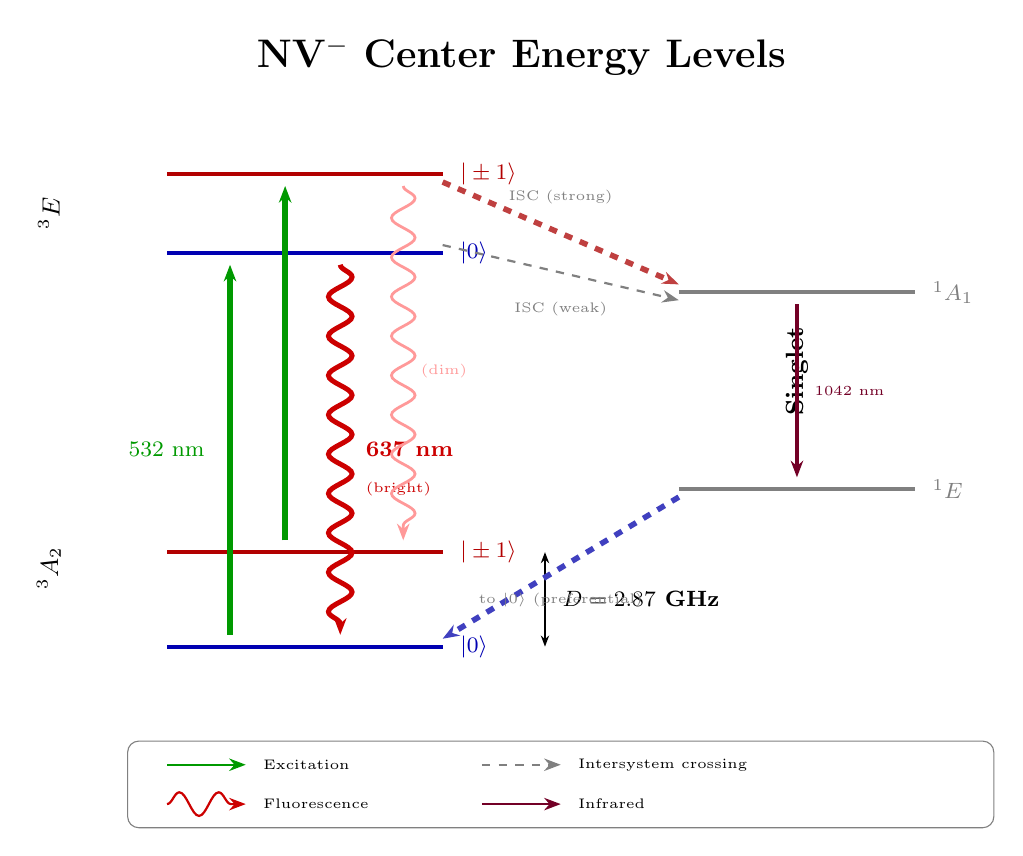
\begin{tikzpicture}[
    level/.style={thick, line width=1.5pt},
    photon/.style={-{Stealth[length=6pt]}, decorate, decoration={snake, amplitude=1.5mm, segment length=5mm}, thick},
    transition/.style={-{Stealth[length=6pt]}, thick},
    isc/.style={-{Stealth[length=6pt]}, dashed, thick, gray},
    label/.style={font=\footnotesize},
]

% === Ground State Triplet (3A2) ===
\node[font=\bfseries\small, rotate=90] at (-1.5, 1) {${}^3A_2$};

% |0> ground
\draw[level, blue!70!black] (0, 0) -- (3.5, 0);
\node[right, label, blue!70!black] at (3.6, 0) {$|0\rangle$};

% |+/-1> ground
\draw[level, red!70!black] (0, 1.2) -- (3.5, 1.2);
\node[right, label, red!70!black] at (3.6, 1.2) {$|\pm1\rangle$};

% ZFS bracket
\draw[{Stealth[length=4pt]}-{Stealth[length=4pt]}, thick] (4.8, 0) -- (4.8, 1.2);
\node[right, font=\footnotesize\bfseries] at (4.9, 0.6) {$D = 2.87$ GHz};

% === Excited State Triplet (3E) ===
\node[font=\bfseries\small, rotate=90] at (-1.5, 5.5) {${}^3E$};

% |0> excited
\draw[level, blue!70!black] (0, 5) -- (3.5, 5);
\node[right, label, blue!70!black] at (3.6, 5) {$|0\rangle$};

% |+/-1> excited
\draw[level, red!70!black] (0, 6) -- (3.5, 6);
\node[right, label, red!70!black] at (3.6, 6) {$|\pm1\rangle$};

% === Singlet States ===
\node[font=\bfseries\small, rotate=90] at (8, 3.5) {Singlet};

% 1A1
\draw[level, gray] (6.5, 4.5) -- (9.5, 4.5);
\node[right, label, gray] at (9.6, 4.5) {${}^1A_1$};

% 1E
\draw[level, gray] (6.5, 2) -- (9.5, 2);
\node[right, label, gray] at (9.6, 2) {${}^1E$};

% === Optical Transitions ===

% Green excitation from |0>
\draw[transition, green!60!black, line width=2pt]
    (0.8, 0.15) -- (0.8, 4.85);
\node[left, font=\footnotesize, green!60!black] at (0.6, 2.5) {532 nm};

% Green excitation from |+/-1>
\draw[transition, green!60!black, line width=2pt]
    (1.5, 1.35) -- (1.5, 5.85);

% Red fluorescence from |0> (BRIGHT)
\draw[photon, red!80!black, line width=1.8pt]
    (2.2, 4.85) -- (2.2, 0.15);
\node[right, font=\footnotesize\bfseries, red!80!black] at (2.4, 2.5) {637 nm};
\node[right, font=\tiny, red!80!black] at (2.4, 2.0) {(bright)};

% Red fluorescence from |+/-1> (DIM)
\draw[photon, red!40!white, line width=1pt]
    (3.0, 5.85) -- (3.0, 1.35);
\node[right, font=\tiny, red!40!white] at (3.1, 3.5) {(dim)};

% === Intersystem Crossing (ISC) ===

% |+/-1> excited -> singlet 1A1 (strong ISC)
\draw[isc, line width=2pt, red!50!gray]
    (3.5, 5.9) -- (6.5, 4.6);
\node[above, font=\tiny, gray] at (5, 5.5) {ISC (strong)};

% |0> excited -> singlet (weak ISC)
\draw[isc, line width=0.8pt]
    (3.5, 5.1) -- (6.5, 4.4);
\node[below, font=\tiny, gray] at (5, 4.5) {ISC (weak)};

% Singlet 1A1 -> 1E (infrared)
\draw[transition, purple!60!black, line width=1.5pt]
    (8, 4.35) -- (8, 2.15);
\node[right, font=\tiny, purple!60!black] at (8.1, 3.25) {1042 nm};

% Singlet 1E -> |0> ground (preferential)
\draw[isc, line width=2pt, blue!50!gray]
    (6.5, 1.9) -- (3.5, 0.1);
\node[below, font=\tiny, gray] at (5, 0.8) {to $|0\rangle$ (preferential)};

% === Title ===
\node[font=\Large\bfseries] at (4.5, 7.5) {NV$^-$ Center Energy Levels};

% === Legend box ===
\begin{scope}[shift={(0, -2)}]
    \draw[rounded corners, thin, gray] (-0.5, -0.3) rectangle (10.5, 0.8);
    \draw[transition, green!60!black, thick] (0, 0.5) -- (1, 0.5);
    \node[right, font=\tiny] at (1.1, 0.5) {Excitation};
    \draw[photon, red!80!black] (0, 0) -- (1, 0);
    \node[right, font=\tiny] at (1.1, 0) {Fluorescence};
    \draw[isc] (4, 0.5) -- (5, 0.5);
    \node[right, font=\tiny] at (5.1, 0.5) {Intersystem crossing};
    \draw[transition, purple!60!black] (4, 0) -- (5, 0);
    \node[right, font=\tiny] at (5.1, 0) {Infrared};
\end{scope}

\end{tikzpicture}
\end{document}
